\documentclass[a4paper,14pt]{extarticle}

\usepackage[T2A]{fontenc}			
\usepackage[utf8]{inputenc}			
\usepackage[english,russian]{babel}

\usepackage[
bookmarks=true, colorlinks=true, unicode=true,
urlcolor=black,linkcolor=black, anchorcolor=black,
citecolor=black, menucolor=black, filecolor=black,
]{hyperref}

\usepackage{color}
\usepackage{caption}
\DeclareCaptionFont{white}{\color{black}}
\DeclareCaptionFormat{listing}{\colorbox{white}{\parbox{\textwidth}{#1#2#3}}}
\captionsetup[lstlisting]{format=listing,labelfont=white,textfont=white}

\usepackage{amsmath,amsfonts,amssymb,amsthm,mathtools} 
\usepackage{wasysym}

%\usepackage[cache=false]{minted}

\usepackage{graphicx}
\usepackage{cmap}
\usepackage{indentfirst}

\usepackage{longtable}

\usepackage{listings} 
\usepackage{fancyvrb}

\usepackage{geometry}
\geometry{left=2cm}
\geometry{right=1.5cm}
\geometry{top=1cm}
\geometry{bottom=2cm}

\setlength{\parindent}{5ex}
\setlength{\parskip}{0.5em}

\usepackage{color}
\usepackage[cache=false, newfloat]{minted}
\newenvironment{code}{\captionsetup{type=listing}}{}
\SetupFloatingEnvironment{listing}{name=Листинг}
 
 
 \begin{document}
 	
 	\def\figurename{Рисунок}
 	
 	\begin{minipage}{0.2\textwidth}
 		\includegraphics[scale=0.05]{img/bmstu.png}
 	\end{minipage}
 	\begin{minipage}{0.7\textwidth}
 		\small
 		\begin{center}
 			\textbf{Министерство науки и высшего образования Российской Федерации}
 			
 			\textbf{Федеральное государственное бюджетное образовательное учреждение высшего образования «Московский государственный технический университет имени Н.Э. Баумана}
 			
 			\textbf{(национальный исследовательский университет)»}
 			
 			\textbf{(МГТУ им. Н.Э. Баумана)}
 		\end{center}
 	\end{minipage}
 	
 	\vspace*{5mm}
 	
 	\normalsize
 	\begin{flushleft}
 		Факультет: <<Информатика и системы управления>>
 		
 		Кафедра: <<Программное обеспечение ЭВМ и информационные технологии>>
 	\end{flushleft}
 	
 	\vspace*{30mm}
 	
 	\LARGE
 	\begin{center}
 		\textbf{Расчетно-пояснительная записка}
 		
 		%	\textbf{к курсовому проекту на тему:}
 		\textbf{к курсовой работе на тему:}
 		
 		\textbf{<<Многопользовательская игра <<Квадраты>>>>}
 	\end{center}
 	
 	\vspace*{15mm}
 	
 	\large
 	\begin{flushleft}
 		\textbf{Студент:} Левушкин И. К. \\
 		\textbf{Группа:} ИУ7-72Б \\
 		%        \textbf{Оценка (баллы):} \\
 		\textbf{Научный руководитель:} Рогозин Н.О.
 	\end{flushleft}
 	
 	\vspace*{50mm}
 	
 	\large
 	\begin{center}
 		Москва, 2020 г.
 	\end{center}
 	
 	\thispagestyle{empty}
 	
 	\newpage
 	
 	\section*{Задание на курсовой проект}
 	
 	Реализовать многопользовательскую игру с определенными правилами. Пользователь должен иметь возможность зарегистрироваться, авторизовываться, добавлять и удалять друзей из списка друзей, приглашать друзей в игру, начинать игру с другом, пригласившим пользователя, а также с пользователем, находящимся в общем списке ждущих игроков. Соответственно, пользователь также должен иметь возможность просматривать этот список и добавляться в него.
 	
 	
 	
 	\newpage
 	
 	\tableofcontents
 	\newpage
 	\section*{Введение}
 	\addcontentsline{toc}{section}{Введение}
 	
 	Сетевые многопользовательские игры занимают значительную нишу в современной игровой индустрии. Число игроков и суммы денег, вращающиеся в этой области, поражают воображение. В 2014 году в «League of Legends» ежемесячно заходили 67 миллионов игроков. В 2015-м на чемпионате мира по игре в <<Dota 2>> призовой фонд составил более 16 миллионов долларов ~\cite{games}.
 	
 	Целью данного проекта является создание сетевой многопользовательской настольной игры <<Квадраты>>.
 	
 	\newpage
 	
 	\section{Аналитический раздел}
 	
 	\subsection{Формализация задачи}
 	
 	В соответствии с техническим заданием необходимо разработать систему, позволяющую первоначально осуществлять регистрацию учетной записи и вход в нее.
 	
 	Далее авторизованный пользователь может проводить стандартные CRUD-операции (создание, просмотр, редактирование, удаление) над определенными сущностями.
 	
 	А именно:
 	\begin{itemize}
 		\item просмотр и редактирование сущности списка друзей;
 		\item просмотр и редактирование сущности пула игроков;
 		\item просмотр, создание и редактирование сущности игры;
 	\end{itemize}
 
 	Авторизованный пользователь с правами администратора будет получать дополнительные возможности:
 	\begin{itemize}
 		\item просмотр, редактирование сущности пользователя;
 		\item редактирование и удаление сущности игры;
 	\end{itemize}
 	
 	Для достижения цели необходим анализ существующих принципов построения веб-приложений.
 	
 	\subsection{Протоколы прикладного уровня}
 	
 	\subsubsection{HTTP}
 	
 	HTTP — протокол прикладного уровня передачи данных, изначально — в виде гипертекстовых документов в формате HTML, в настоящее время используется для передачи произвольных данных ~\cite{http}.
 	
 	HTTP явялется наиболее распространенным протоколом всемирной паутины (World Wide Web) ~\cite{www}. Основным объектом манипуляции в HTTP является ресурс, на который указывает URI (Uniform Resource Identifier – уникальный идентификатор ресурса) в запросе клиента. Основными ресурсами являются хранящиеся на сервере файлы, но ими могут быть и другие логические или абстрактные объекты. Протокол HTTP позволяет указать способ представления (кодирования) одного и того же ресурса по различным параметрам: MIME-типу, языку и т. д. Благодаря этой возможности клиент и веб-сервер могут обмениваться двоичными данными, хотя данный протокол является текстовым.
 	
 	Существует несколько версий этого протокола: HTTP 1.0, HTTP 1.1, НТТР/2 и НТТР/3. Для транспортировки HTTP-сообщений служит протокол TCP (обычно 80 порт).
 	
 	Структура протокола определяет, что каждое HTTP-сообщение состоит из трёх частей, которые передаются в следующем порядке:
 	
 	\begin{enumerate}
 		\item стартовая строка — определяет тип сообщения;
 		\item заголовки  — характеризуют тело сообщения, параметры передачи и прочие сведения;
 		\item тело сообщения — непосредственно данные сообщения. Обязательно должно отделяться от заголовков пустой строкой.
 	\end{enumerate}
 
 	\subsubsection{HTTPS}
 	
 	HTTPS — расширение протокола HTTP, поддерживающее шифрование. Данные, передаваемые по протоколу HTTP, <<упаковываются>> в криптографический протокол SSL или TLS, тем самым обеспечивается защита этих данных. В отличие от HTTP, для HTTPS по умолчанию используется TCP-порт 443. Эта система была разработана компанией Netscape Communications Corporation, чтобы обеспечить аутентификацию и защищённое соединение. HTTPS широко используется во всемирной паутине для приложений, в которых важна безопасность соединения, например, в платежных системах.
 	
 	SSL/TLS-сертификат — это цифровая подпись сайта. С помощью сертификата подтверждается подлинность сайта. Перед тем как установить защищённое соединение, браузер запрашивает этот документ и обращается к центру сертификации, чтобы подтвердить легальность документа. Если он действителен, то браузер считает этот сайт безопасным и начинает обмен данными.
 	
 	В настоящее время HTTPS поддерживается всеми популярными браузерами.
 	
 	\subsection{Архитектура}
 	
 	\subsubsection{Клиент-серверная архитектура}
 	
 	Клиент-серверная архитектура — вычислительная или сетевая архитектура, в которой задания или сетевая нагрузка распределены между поставщиками услуг, называемыми серверами, и заказчиками услуг, называемыми клиентами. Фактически клиент и сервер — это программное обеспечение. Обычно эти программы расположены на разных вычислительных машинах и взаимодействуют между собой через вычислительную сеть посредством сетевых протоколов, но они могут быть расположены также и на одной машине ~\cite{client-server}.
 	
 	\begin{figure}[h!]
 		\begin{center}
 			{\includegraphics[scale = 0.6]{img/client-server.jpeg}}
 			\label{ris:client-server}
 		\end{center}
 		\caption{Клиент-серверная архитектура.}
 	\end{figure}
 
 	\subsubsection{REST архитектура}
 	
 	REST — архитектурный стиль взаимодействия компонентов распределённого приложения в сети ~\cite{rest}. REST представляет собой согласованный набор ограничений, учитываемых при проектировании распределённой системы. В определённых случаях (интернет-магазины, поисковые системы, прочие системы, основанные на данных) это приводит к повышению производительности и упрощению архитектуры. В широком смысле компоненты в REST взаимодействуют наподобие взаимодействия клиентов и серверов во Всемирной паутине.
 	
 	Ограничения REST:
 	
 	\begin{itemize}
 		\item модель клиент-сервер; 
 		\item отсутствие состояния;
 		\item кэширование;
 		\item единообразие интерфейса:
 			\begin{itemize}
 				\item идентификация ресурсов;
 				\item манипуляция ресурсами через представление;
 				\item <<самоописываемые>> сообщения;
 				\item гипермедиа как средство изменения состояния приложения;
 			\end{itemize}
 		\item слои.
 	\end{itemize}
 
 	Для веб-служб, построенных с учётом REST (то есть не нарушающих накладываемых им ограничений), применяют термин <<RESTful>>.
 	
 	Рой Филдинг — один из главных авторов спецификации протокола HTTP, описывает влияние архитектуры REST на масштабируемость следующим образом:
 	
 	\begin{itemize}
 		\item простота унифицированного интерфейса;
 		\item открытость компонентов к возможным изменениям для удовлетворения изменяющихся потребностей (даже при работающем приложении);
 		\item прозрачность связей между компонентами системы для сервисных служб;
 		\item переносимость компонентов системы путем перемещения программного кода вместе с данными;
 		\item надёжность, выражающаяся в устойчивости к отказам на уровне системы при наличии отказов отдельных компонентов, соединений или данных.
 	\end{itemize}
 
 	\subsubsection{Монолитная архитектура}
 	
 	В программной инженерии монолитная модель относится к единой неделимой единице. Концепция монолитного программного обеспечения заключается в том, что различные компоненты приложения объединяются в одну программу на одной платформе. Обычно монолитное приложение состоит из базы данных, клиентского пользовательского интерфейса и серверного приложения. Все части программного обеспечения унифицированы, и все его функции управляются в одном месте ~\cite{mono}.
 	
 	Большим преимуществом монолита является то, что его легко реализовать. В монолитной архитектуре можно быстро начать реализовывать бизнес-логику вместо того, чтобы тратить время на размышления о межпроцессном взаимодействие.
 	
 	Однако в монолите практически нет изоляции. Проблема или ошибка в модуле может замедлить или разрушить все приложение.
 	
 	\subsubsection{Микросервисная архитектура}
 	
 	Микросервисная архитектура — вариант сервис-ориентированной архитектуры программного обеспечения, направленный на взаимодействие насколько это возможно небольших, слабо связанных и легко изменяемых модулей — микросервисов.
 	
 	Микросервисы легче держать модульными. Технически это обеспечивается жесткими границами между отдельными сервисами.
 	
 	В больших компаниях разные сервисы могут принадлежать разным командам. Услуги могут быть повторно использованы всей компанией. Это также позволяет командам работать над услугами в основном самостоятельно. Нет необходимости координировать развертывание между командами. Развивать сервисы лучше с увеличением количества команд.
 	
 	На рисунке 2 показаны различия между монолитной архитектурой и микросервисной.
 	
 	\begin{figure}[h!]
 		\begin{center}
 			{\includegraphics[scale = 0.5]{img/mono-micro.png}}
 			\label{ris:mono-micro}
 		\end{center}
 		\caption{Монолитная и микросервисная архитектуры.}
 	\end{figure}
 
 	\subsection{Базы данных}
 	
 	\subsubsection{Общие сведения}
 	
 	Очевидно, клиентские данные нужно каким-то образом хранить, поэтому требуется анализ существующих типов баз данных. Рассмотрим популярные и зарекомендовавшие себя решения – реляционную и нереляционную. Помимо этих видов существуют и другие (иерархическая, сетевая) ~\cite{bd}, но выбранные БД являются наиболее популярными в мире веба.
 	
 	\subsubsection{Реляционная модель}
 	
 	Реляционная модель данных использует организацию данных в виде двумерных таблиц. Каждая такая таблица, называемая реляционной таблицей или отношением, представляет собой двумерный массив и обладает следующими свойствами: все столбцы в таблице однородные, т.е. все элементы в одном столбце имеют одинаковый тип и максимально допустимый размер; каждый столбец имеет уникальное имя; одинаковые строки в таблице отсутствуют; порядок следования строк и столбцов в таблице не имеет значения. Основными структурными элементами реляционной таблицы являются поле и запись.
 	
 	Поле в таблице, называемое внешним ключом, может содержать ссылки на столбцы в других таблицах, что позволяет их соединять.
 	
 	Ниже приведен пример организации данных курьерской службы приведен на рисунке 3.
 	
 	\newpage
 	
 	\begin{figure}[h!]
 		\begin{center}
 			{\includegraphics[scale = 0.6]{img/deliver.png}}
 			\label{ris:deliver}
 		\end{center}
 		\caption{Пример реляционной модели.}
 	\end{figure}
	
 
 	Для доступа к данным используется язык структурированных запросов (SQL) ~\cite{sql}. Реляционная модель – надежный выбор для многих приложений, один из старейших способов организации информации и самый популярный.
 	
 	Сложности состоят в изначальном проектировании такой БД, ведь при плохо спроектированной системе возможно значительное снижение скорости доступа к данным, стремительное разрастание занимаего пространства и другие проблемы, связанные с поддержкой и модификацией программы.

 	\subsubsection{Нереляционная модель}
 	
 	NoSQL – группа типов БД, предлагающих подходы, отличные от стандартного реляционного шаблона ~\cite{nosql}. Говоря NoSQL, подразумевают либо <<не-SQL>>, либо <<не только SQL>>, чтобы уточнить, что иногда допускается SQL-подобный запрос.
 	
 	Описание схемы данных в случае использования NoSQL-решений может осуществляться через использование различных структур данных: хеш-таблиц, деревьев и других.
 	
 	Вместе с достоинствами в виде гибкости системы имеются и недостатки, связанные с отсутствием жесткой схемы отношения между данными. Кроме того, зачастую нереляционные БД привязаны к конкретной СУБД и требуют специализированных знаний для работы с ними, в то время как реляционная модель точно имеет поддержку общего стандарта написания запросов.
 	
 	\subsection*{Выводы по аналитическому разделу}
 	
 	В рамках данной работы было решено использовать реляционную модель организации данных, поскольку она остается надежным выбором для многих систем и основана на строгом математическом аппарате, что позволяет лаконично описывать необходимые операции над данными.
 	
 	В результате проведенного анализа было решено разрабатывать веб-приложение в клиент-серверной архитектуре, используя методологию REST, что позволит сделать ПО надежным и легко масштабируемым.
 	
 	Сервер будет представлять собой монолитную архитектуру, поскольку является наилучшим решением для небольших проектов.
 	
 	\newpage
 	
 	\section{Конструкторский раздел}
 	
 	\subsection{Правила игры}
 	
 	В данной работе реализуется логическая настольная игра с полной информацией ~\cite{game}, что означает, что игра игрокам известны функция полезности, правила игры, а также ходы других игроков.
 	
 	\subsubsection{Инвентарь}
 	
 	В игру <<Квадраты>> играют на квадратной доске, расчерченной вертикальными и горизонтальными линиями. Стандартная доска имеет размер поля 11x11, но также возможны любые другие вариации. У каждого из игроков имеется неограниченное количество фишек его цвета, который присваивается ему в начале игры.
 	
 	\subsubsection{Основные правила}
 	
 	Играют в игру два игрока, один из которых получает красные фишки, другой - синие. Цель игры - набрать количество очков большее чем у противника.
 	
 	\subsubsection{Начальная позиция}
 	
 	Перед началом игры доска пуста. Первыми ходят синие. Затем красные. Далее ходы делаются по очереди. 
 	
 	Игрок не может отказываться от хода.
 	
 	\subsubsection{Порядок игры}
 	
 	Делая ход, игрок выставляет одну фишку на доску в любую незанятую клетку. Фишки, однажды поставленные на доску, не убираются. За каждый собранный <<квадрат>> на поле игрок получает определенное количество очков в зависимости от величины стороны квадрата.
 	
 	Квадрат представляет собой конструкцию, соединенную в углах четырьмя фишками одного цвета. Соединение квадратов по горизонтали-вертикали дает $1, 3, 5, 7, 9...$ очков в зависимости от длины стороны квадрата. Соединение квадратов по диагонали дает $2, 4, 6, 8, 10,...$ очков в зависимости от длины стороны квадрата. 
 	
 	Конструкция, состоящая из 4 фишек одного цвета, у которой все ребра равны, и {\bf имеющая} или нет внутри себя или между фишек другие фишки, называется {\bf квадратом}.
 	
 	\subsubsection{Завершение партии}
 	
 	Партия заканчивается, как только поле будет полностью заполнено фишками. Победителем определяется игрок, набравший наиболее количество очков.
 	
 	\newpage
 	
 	\subsection{Описание функционала}
 	
 	Формулировка требования к возможностям программного обеспечения из раздела 1.1 требует большей конкретики. Диаграмма вариантов использования (Use-Case) описывает взаимоотношения и зависимости между вариантами использования и действующими лицами, участвующими в процессе.
 	
 	\begin{figure}[h!]
 		\begin{center}
 			{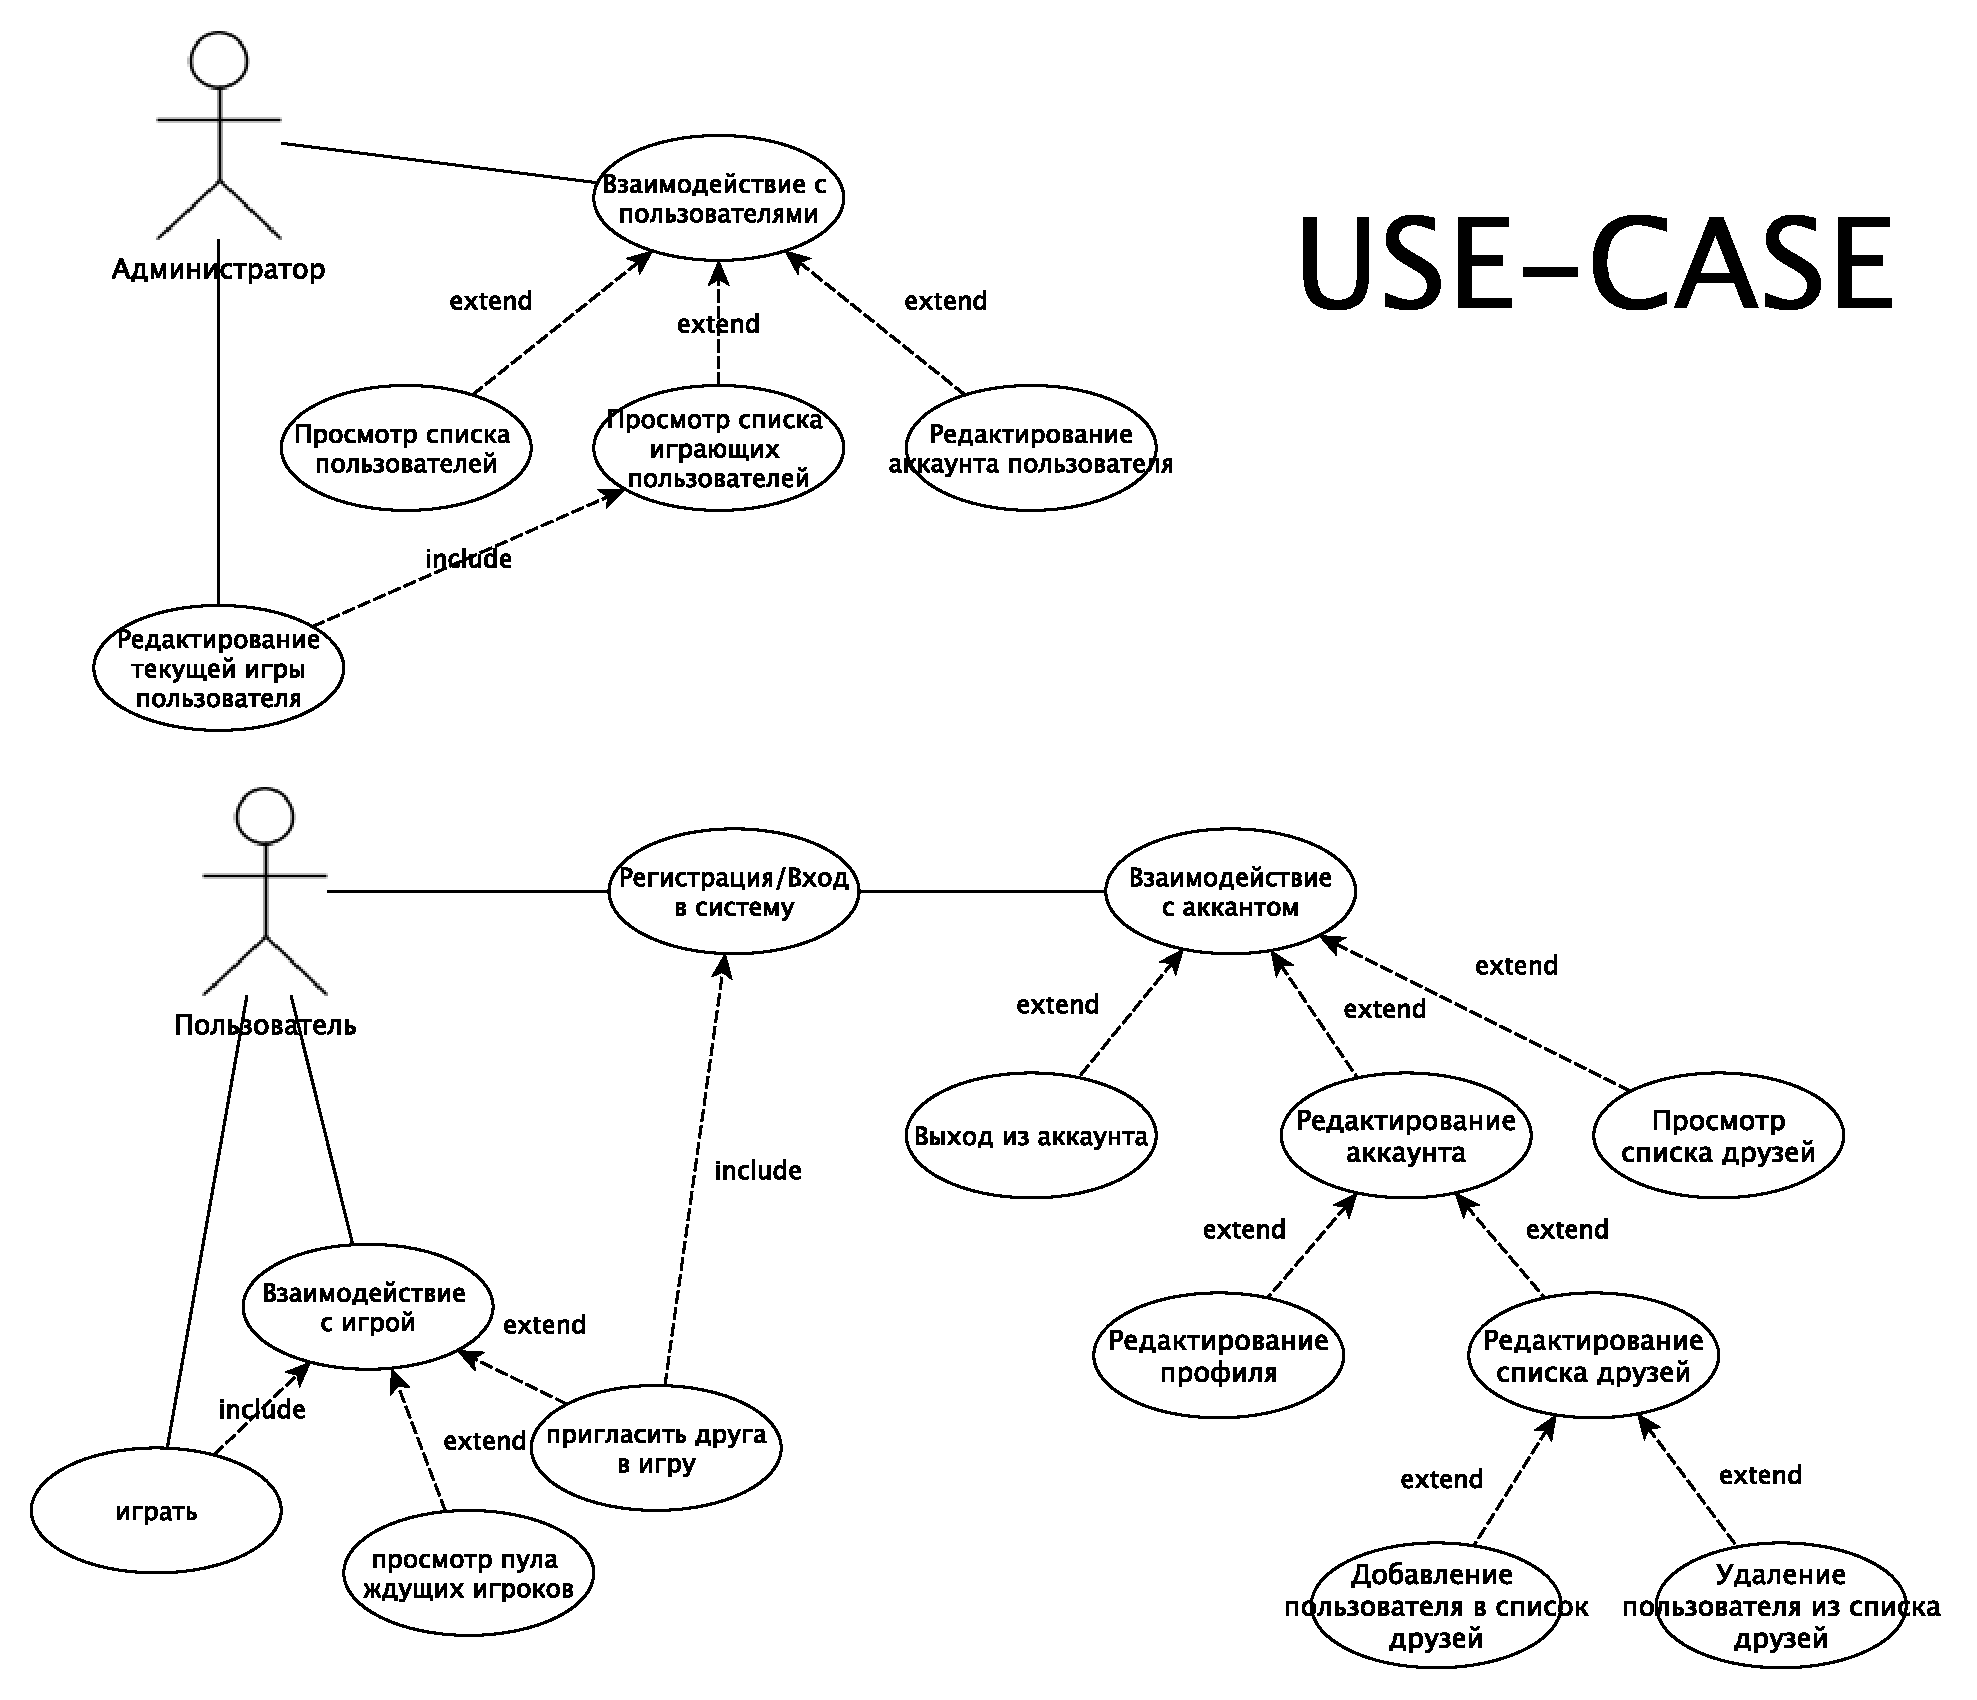
\includegraphics[scale = 0.5]{img/use-case.pdf}}
 			\label{ris:use-case}
 		\end{center}
 		\caption{Use-Case диаграмма.}
 	\end{figure}
 	
 	\newpage
 
 	\subsection{Структура базы данных}
 	
 	Ниже приведены диаграмма <<сущность-связь>> (ER), описывающая концептуальную схему предметной области, и диаграмма сущностей спроектированной базы данных, графическое изображение которой дает четкое представление о действующих сущностях и их атрибутах.
 	
 	\begin{figure}[h!]
 		\begin{center}
 			{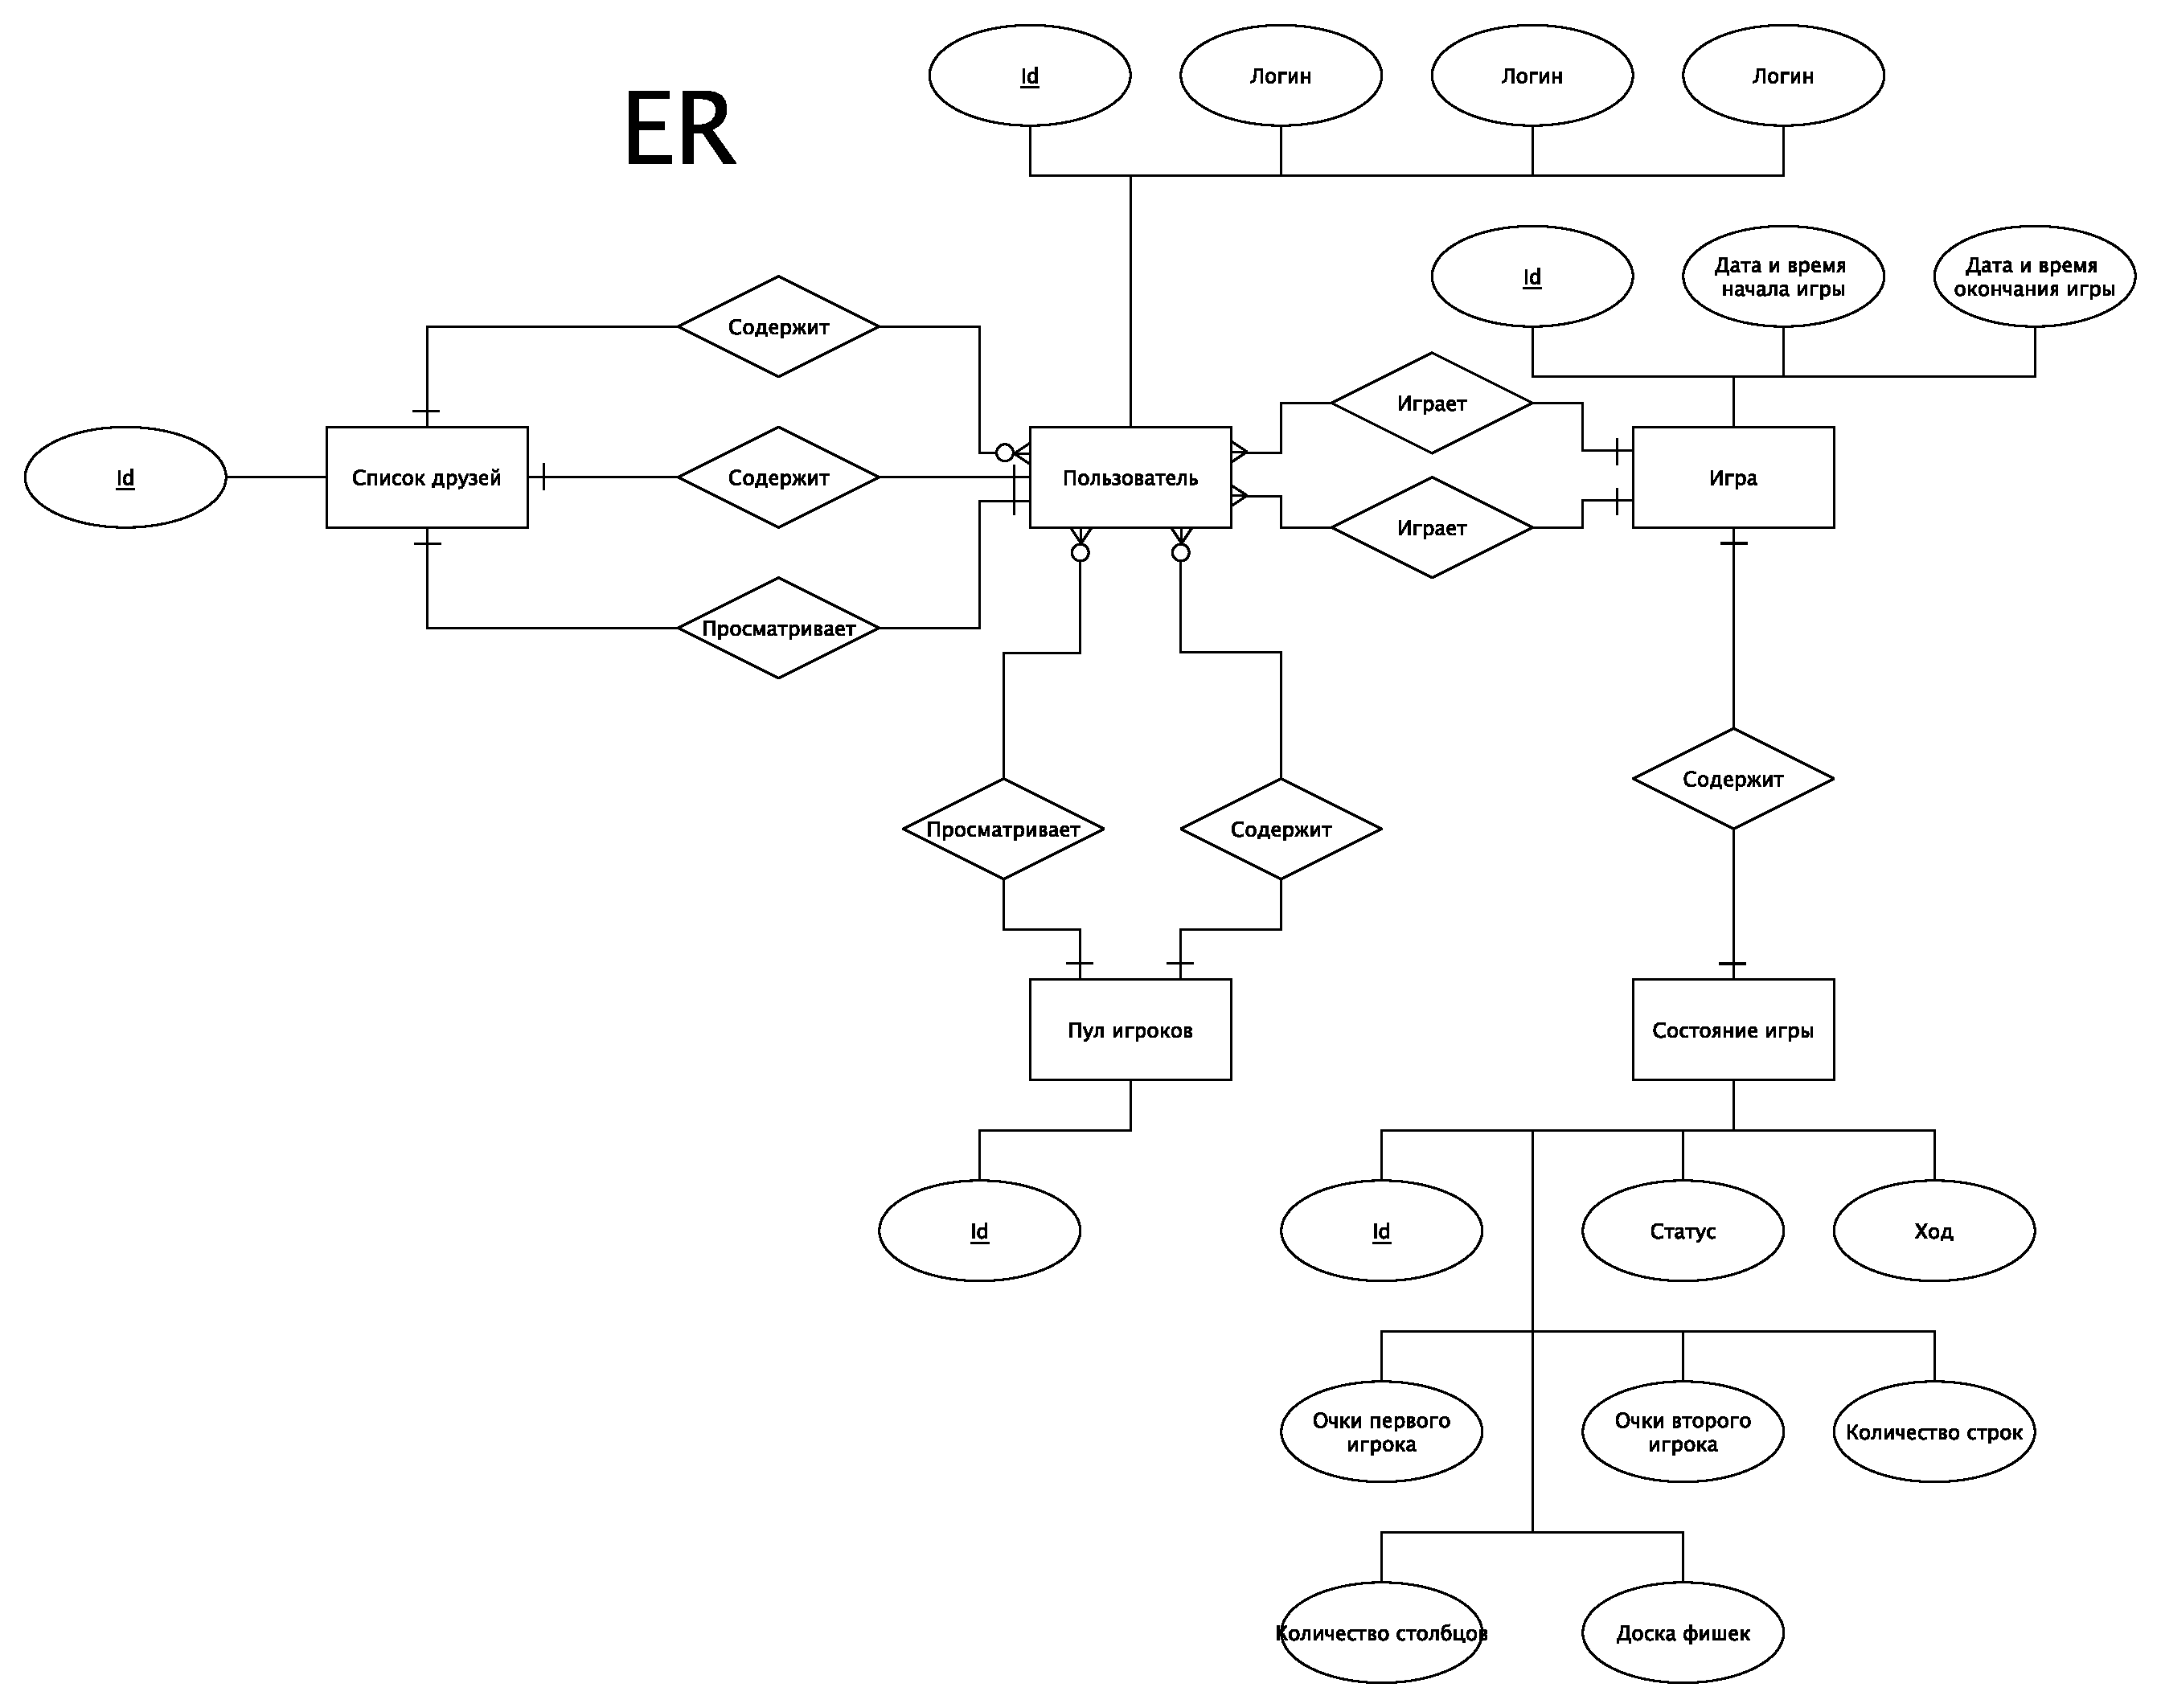
\includegraphics[scale = 0.4]{img/er.pdf}}
 			\label{ris:er}
 		\end{center}
 		\caption{ER диаграмма.}
 	\end{figure}
 
 	\newpage
 
 	\begin{figure}[h!]
 		\begin{center}
 			{\includegraphics[scale = 0.35]{img/database_diagram.png}}
 			\label{ris:bd}
 		\end{center}
 		\caption{Диаграмма базы данных.}
 	\end{figure}
 
 	\subsection{API системы в идеологии REST}
 	
 	Грамотным решением является отделение логики программы для последующего удобного взаимодействия с ней и возможности переиспользования (построение API).
 	
 	Ниже приведено краткое описание спроектированного API системы в идеологии REST в формате Swagger:
 	
 	\begin{figure}[h!]
 		\begin{center}
 			{\includegraphics[scale = 0.35]{img/user.png}}
 			\label{ris:user}
 		\end{center}
 		\caption{API сущности пользователя (user).}
 	\end{figure}
 
 	\newpage
 
 	\begin{figure}[h!]
 		\begin{center}
 			{\includegraphics[scale = 0.4]{img/friend.png}}
 			\label{ris:friend}
 		\end{center}
 		\caption{API сущности друга (friend).}
 	\end{figure}
 
 	\begin{figure}[h!]
 		\begin{center}
 			{\includegraphics[scale = 0.4]{img/pull.png}}
 			\label{ris:pull}
 		\end{center}
 		\caption{API сущности пула игроков (pull).}
 	\end{figure}
 
 	\begin{figure}[h!]
 		\begin{center}
 			{\includegraphics[scale = 0.4]{img/game.png}}
 			\label{ris:game}
 		\end{center}
 		\caption{API сущности игры (game).}
 	\end{figure}
 	 
 	\subsection{Описание классов и компонентов}
 	
 	Общее представление компонентов программы содержится на рисунке 11.
 	
 	\newpage
 	
 	\begin{figure}[h!]
 		\begin{center}
 			{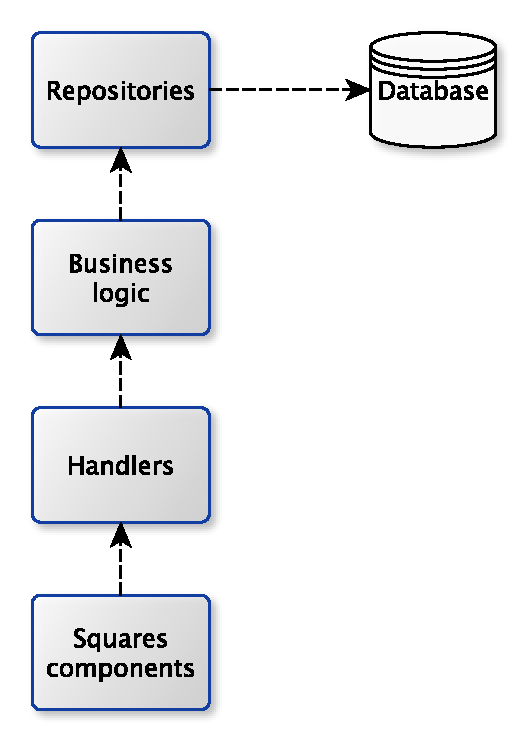
\includegraphics[scale = 0.6]{img/theme.pdf}}
 			\label{ris:theme}
 		\end{center}
 		\caption{Диаграмма компонентов.}
 	\end{figure}
 	
 	Ниже приведена диаграмма классов бизнес-логики.
 	
 	\begin{figure}[h!]
 		\begin{center}
 			{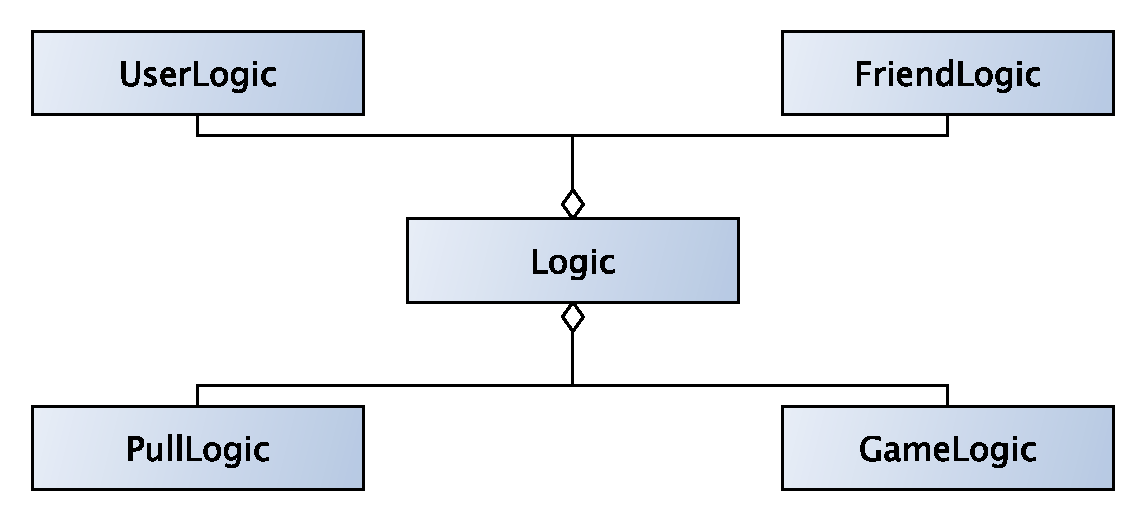
\includegraphics[scale = 0.4]{img/logic.pdf}}
 			\label{ris:logic}
 		\end{center}
 		\caption{Диаграмма классов бизнес-логики.}
 	\end{figure}
 	
 	Аналогично слою бизнес-логики строятся компоненты обработки запросов и репозитория. Такая структура, на первый взгляд, выглядит избыточной, но позволяет абстрагировать уровни приложения и легче его тестировать.
 	
 	\newpage
 	
 	Ниже представлена функциональная модель системы.
 	
 	\begin{figure}[h!]
 		\begin{center}
 			{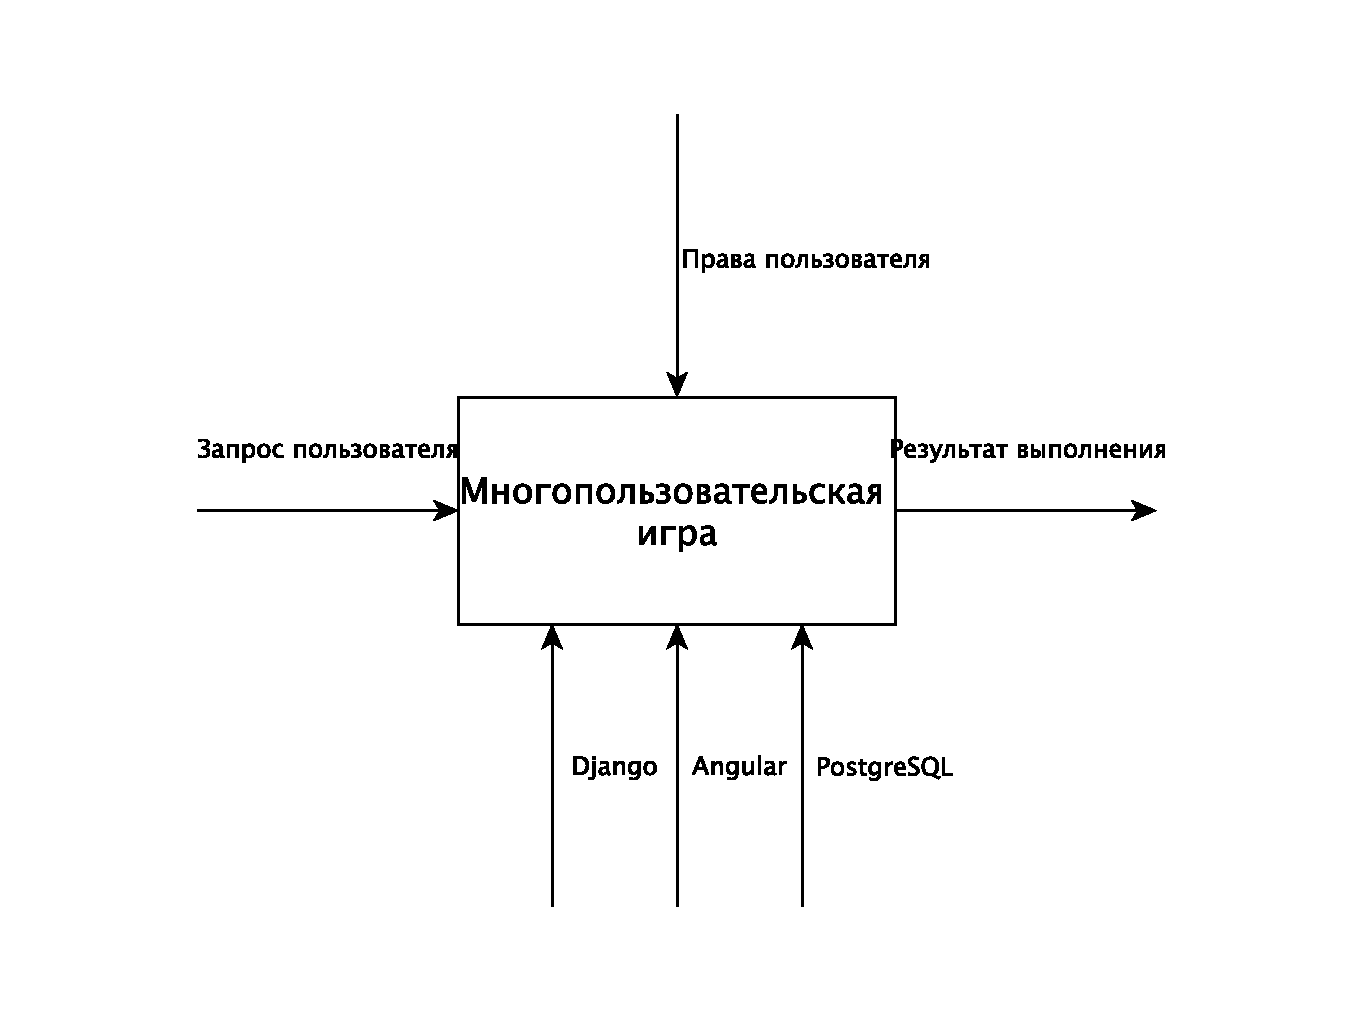
\includegraphics[scale = 0.4]{img/func.pdf}}
 			\label{ris:func}
 		\end{center}
 		\caption{Функциональная модель системы.}
 	\end{figure}
 	
 	\subsection*{Выводы по конструкторскому разделу}
 	
 	Были спроектированы и представлены описание функционала программного обеспечения в виде Use-Case диаграммы, структура базы данных с помощью ER-диаграммы и диаграммы базы данных, API системы в идеологии REST, а также дано описание классов и компонентов системы.
 	
 	\newpage
 	
 	\section{Технологический раздел}
 	
 	\subsection{Использованные технологии}
 	
 	Основной используемой технологией для построения серверной части приложения выбран веб-фреймворк Django ~\cite{django}. Django – это веб- фреймворк языка Python ~\cite{python}, использующий шаблон проектирования MVC.
 	
 	Для построения клиентской части приложения выбран фреймворк Angular ~\cite{angular}, использующий язык TypeScript ~\cite{ts}.
 	
 	В качестве системы управления базами данных используется PostgreSQL ~\cite{postgresql}. Фундаментальная характеристика представленной СУБД – это поддержка пользовательских объектов и их поведения. Это делает PostgreSQL невероятно гибким и надежным. Среди прочего, здесь можно создавать, хранить и извлекать сложные структуры данных.
 	
 	Ниже представлен основной технологический стек проекта.
 	
 	\textit{\bf Front-end:}
 	\begin{itemize}
 		\item Язык гипертекстовой разметки HTML5\cite{html}
 		\item Таблицы стилей CSS3\cite{css}
 		\item Язык программирования TypeScript\cite{ts}
 	\end{itemize}
 	
 	\textit{\bf Back-end:}
 	\begin{itemize}
 		\item СУБД PostgreSQL\cite{postgresql}
 		\item Фреймворк Django\cite{django}
 		\item Язык программирования Python3\cite{python}
 	\end{itemize}
 
 	\newpage
 	
 	\subsection{Примеры кода ПО}
 	
 	Организацию серверной и клиентской частей можно проследить на примере одной из сущностей. Для демонстрации возьмем структуру проекта, показанную в листинге 1.
 	
 	\begin{listing}
 		\caption{Модель доступа к данным сущности pull}
 		\label{code:pull_model}
 		\begin{minted}[frame=single,framerule=2pt, fontsize=\footnotesize]{python}
from django.db import models
from .users import Users
from ..managers import PullPlayersManager

from datetime import datetime


class PullPlayers(models.Model):
	player = models.OneToOneField(Users, on_delete=models.PROTECT)
	
	date_time_appear = models.DateTimeField(default=datetime.now)
	
	objects = PullPlayersManager()
	
	def __str__(self):
		return self.player.user.username
 		\end{minted}
 	\end{listing}
 
 
 	Принципы чистой архитектуры указывают на разделение кода на независимые слои. На примере метода добавления пользователя в пул игроков можно просмотреть, как это соблюдается в текущей реализации. 
 	
 	\newpage
 	
 	Листинг 2 содержит post-метод обработчика HTTP-запросов, который выполняет проверку JWT-токена (процедура аутентификации), передает право классу бизнес-логики пула решать, можно ли создавать новую запись в таблице пула игроков, и если ответ положительный, то передает управление классу менеджеру пула, чтоб тот создал новую запись в таблице пула.
 	
 	\begin{listing}
 		\caption{Post-метод pull-обработчика HTTP-запросов}
 		\label{code:pull_view}
 		\begin{minted}[frame=single,framerule=2pt, fontsize=\footnotesize]{python}
from rest_framework.response import Response
from rest_framework import status
from rest_framework import authentication, permissions
from rest_framework.views import APIView

from ..repository import PullPlayersCRUD
from ..serializers import PullPlayersSerializer
from ..business_logic import PullPlayersLogic


class PullPlayersView(APIView):
	manager = PullPlayersCRUD()
	logic = PullPlayersLogic()
	
	authentication_classes = [authentication.TokenAuthentication]
	permission_classes = [permissions.IsAuthenticated]
	
	# добавить себя в пул
	def post(self, request):
		if not self.logic.user_in_pull(request.user.pk):
			self.manager.create_note(request.user.pk)
		else:
 		return Response(f'User is already in pull', status=status.HTTP_403_FORBIDDEN)
 		
 		return Response({"success": f'User was added in pull successfully'},
 		status=status.HTTP_201_CREATED)
 		\end{minted}
 	\end{listing}
 
 	\newpage
 
 	Далее представлен уровень бизнес-логики (листинг 3), где происходит установление принадлежности пользователя к пулу и принятие решения в соответсвующии с результатом.
 	
 	\begin{listing}
 		\caption{Pull-бизнес-логика}
 		\label{code:pull_logic}
 		\begin{minted}[frame=single,framerule=2pt, fontsize=\footnotesize]{python}
from ..models import PullPlayers
from .user import UsersLogic

from ..repository import UsersCRUD

class PullPlayersLogic:

	def __init__(self):
		self.objects = PullPlayers.objects
		self.users_logic = UsersLogic()
		self.users_manager = UsersCRUD()
	
	
	def user_is_admin(self, user):
		return self.users_logic.user_is_admin(user)
	
	def user_in_pull(self, user_pk):
		users = self.users_manager.get_note_by_user_pk(user_pk)
		return self.objects.is_user_exists(users.pk)
	
	def user_in_pull2(self, users_pk):
		return self.objects.is_user_exists(users_pk)
 		\end{minted}
 	\end{listing}
 	
 	\newpage
 
 	Ниже идет обращение к методу репозитория, в котором происходит непосредственное взаимодействие с базой данных (листинг 4).
 	
 	\begin{listing}
 		\caption{Репозиторий пула}
 		\label{code:pull_rep}
 		\begin{minted}[frame=single,framerule=2pt, fontsize=\footnotesize]{python}
from ..models import Users, Games, PullPlayers, Friends


class PullPlayersCRUD:

	def __init__(self):
		self.objects = PullPlayers.objects
		self.user_objects = Users.objects
	
	def get_all(self):
		return self.objects.get_all()
	
	def get_note(self, user_pk):
		users = self.user_objects.get_note_by_user_pk(user_pk)
		return self.objects.get_note(users.pk)
	
	def delete_note(self, user_pk):
		users = self.user_objects.get_note_by_user_pk(user_pk)
		self.objects.delete_note(self.user_objects.get_note(users.pk))
	
	def delete_note2(self, users_pk):
		self.objects.delete_note(self.user_objects.get_note(users_pk))
	
	def create_note(self, user_pk):
		users = self.user_objects.get_note_by_user_pk(user_pk)
		return self.objects.create_note(self.user_objects.get_note(users.pk))
 		\end{minted}
 	\end{listing}
 	
 
 	Исходя из представленного кода видно, что слои независимы друг от друга.
 	
 	\subsection{Nginx}
 	
 	Nginx – это веб-сервер с обратным прокси-сервером, который используется для обслуживания динамического содержимого веб- сайта и контроля загрузки сервера ~\cite{nginx}.
 	Основная настройка nginx указана в листинге 5.
 	
 	В секции events настраивается подведение nginx относительно сетевых соединений. Если multi\_accept установлен в on, то рабочий процесс за один раз будет принимать сразу все новые соединения.
 	
 	Значение worker\_connections определяет максимально возможное количество одновременных соединений к серверу.
 	
 	Секция http объединяет все настройки относительно работы протокола http.
 	Параметр sendfile включает или отключает использование сервером одноимённого системного вызова. Включение этого параметра увеличивает производительность nginx за счёт использования более эффективного способа ввода-вывода.
 	
 	Включение опции tcp\_nopush заставляет nginx пытаться отправлять HTTP-заголовки в одном пакете.
 	
 	Параметр tcp\_nodelay влияет разрешает или запрещает использование сервером опции сокета TCP\_NODELAY при работе с постоянными соединениями.
 	
 	Параметр gzip управляет включением/отключением сжатия сервером данных, передаваемых клиенту. Включение этой опции увеличивает нагрузку на центральный процессор системы, однако позволяет существенно сократить объём передаваемых данных.
 	
 	Параметр proxy\_cache\_path позволяет настроить параметры хранения кэша. nginx кэш позволяет значительно сократить количество запросов на бэкенд. Это достигается путем сохранения HTTP ответа, на определенное время, а при повторном обращении к ресурсу, отдачи его из кэша без проксирования запроса на бекенд.
 	
 	При помощи опции default\_type задаётся MIME-тип по умолчанию, который будет передавать сервер клиенту, если этот тип не удалось определить.
 	
 	Параметр access\_log определяет местоположение и формат лог-файла доступа к содержимому.
 	
 	\begin{listing}
 		\caption{Конфигурация nginx}
 		\label{code:nginx}
 		\begin{minted}[frame=single,framerule=2pt, fontsize=\footnotesize]{cfg}
events {
multi_accept on;
worker_connections 1024;
}

http {
charset utf-8;
sendfile on;
tcp_nopush on;
tcp_nodelay on;
server_tokens off;
log_not_found off;
types_hash_max_size 4096;
client_max_body_size 16M;
gzip on;
gzip_comp_level 5;
proxy_cache_path /var/cache/nginx levels=1:2 keys_zone=all:32m max_size=1g;

# MIME
include mime.types;
default_type application/octet-stream;

# logging
log_format  main  '$remote_addr - $remote_user [$time_local] "$request" '
'$status $body_bytes_sent "$http_referer" '
'"$http_user_agent" "$http_x_forwarded_for"';

access_log  /Users/ilalevuskin/github/GitHub/computer_networks/project/nginx/access.log  main;
error_log /Users/ilalevuskin/github/GitHub/computer_networks/project/nginx/error.log warn;

server {
listen 82;
add_header Server Squares always;

location / {
set $do_not_cache 0;
if ($http_cookie ~* ".+" ) {
set $do_not_cache 1;
}
proxy_cache_bypass $do_not_cache;
proxy_pass http://127.0.0.1:81;
proxy_set_header Host $host;
proxy_set_header X-Real-IP $remote_addr;
proxy_set_header X-Forwarded-For $proxy_add_x_forwarded_for;
proxy_cache all;
proxy_cache_methods GET HEAD;
proxy_cache_valid any 1m;
}
}

upstream backend_balanced {
server localhost:8000 weight=2;
server localhost:8001 weight=1;
server localhost:8002 weight=1;
}
}
 		\end{minted}
 	\end{listing}
 
 	Веб-сервер по умолчанию распределяет запросы равномерно между бэкендами (с учетом весов). Этот стандартный метод в Nginx, так что директива включения отсутствует. Веса выбраны так, что из каждых 4 запросов бэкенд \textit{localhost:8000} будет обрабатывать 2, \textit{localhost:8001} 1, а \textit{localhost:8002} 1 (листинг 6).
 	
 	\begin{listing}
 		\caption{Балансировка нагрузки}
 		\label{code:balance}
 		\begin{minted}[frame=single,framerule=2pt, fontsize=\footnotesize]{cfg}
upstream backend_main {
server localhost:8000;
}

map $request_method $backend
{
GET backend_balanced;
HEAD backend_balanced;
default backend_main;
}
 	\end{minted}
 \end{listing}
 	
 	
 	\subsection{Примеры работы серверной части приложения}
 	
 	Ниже приведены примеры запросов и ответов сервера. Тестирование проводилось с помощью утилиты Postman ~\cite{postman}
 	
 	\begin{figure}[h!]
 		\begin{center}
 			{\includegraphics[scale = 0.5]{img/reg.png}}
 			\label{ris:reg}
 		\end{center}
 		\caption{Регистрация пользователя.}
 	\end{figure}
 
 	\newpage
 
 	\begin{figure}[h!]
 		\begin{center}
 			{\includegraphics[scale = 0.5]{img/login.png}}
 			\label{ris:login}
 		\end{center}
 		\caption{Вход пользователя.}
 	\end{figure}
 
 	\begin{figure}[h!]
 		\begin{center}
 			{\includegraphics[scale = 0.5]{img/logout.png}}
 			\label{ris:logout}
 		\end{center}
 		\caption{Выход пользователя.}
 	\end{figure}
 
 	\newpage
 
 	\begin{figure}[h!]
 		\begin{center}
 			{\includegraphics[scale = 0.5]{img/pull2.png}}
 			\label{ris:pull}
 		\end{center}
 		\caption{Просмотр пула игроков.}
 	\end{figure}
 
 	\begin{figure}[h!]
 		\begin{center}
 			{\includegraphics[scale = 0.5]{img/friends.png}}
 			\label{ris:friends}
 		\end{center}
 		\caption{Просмотр списка друзей.}
 	\end{figure}
 
 	\newpage
 
 	\begin{figure}[h!]
 		\begin{center}
 			{\includegraphics[scale = 0.5]{img/create_game.png}}
 			\label{ris:create_game}
 		\end{center}
 		\caption{Создание игры.}
 	\end{figure}
 
 	\begin{figure}[h!]
 		\begin{center}
 			{\includegraphics[scale = 0.5]{img/refresh_game.png}}
 			\label{ris:refresh_game}
 		\end{center}
 		\caption{Обновление игры.}
 	\end{figure}
 
 	\newpage
 
 	\begin{figure}[h!]
 		\begin{center}
 			{\includegraphics[scale = 0.5]{img/delete_game.png}}
 			\label{ris:delete_game}
 		\end{center}
 		\caption{Удаление игры администратором.}
 	\end{figure}
 	
 	\subsection*{Выводы по технологическому разделу}
 	
 	В результате проделанной работы были выбраны технологии для разработки ПО.
 	
 	Были приведены листинги кода ПО и примеры работы серверной части приложения.
 	
 	\newpage
 	\section*{Заключение}
 	\addcontentsline{toc}{section}{Заключение}
 	
 	В ходе проделанной работы был выполнен анализ принципов построения современных веб-приложений.
 	
 	Спроектирована архитектура программы на основе шаблона MVC со стороны сервера. Была использована реляционная модель организации данных. Веб-приложение разрабатывалось, используя методологию REST.

 	Таким образом, с помощью СУБД PostgreSQL и фреймворков Django и Angular было реализовано веб-приложение SPA - многопользовательская игра <<Квадраты>>.
 	
 	В планах дальнейшего развития приложения - расширение функционала, в рамках которого будет реализован список лучших игроков, обмен сообщений между игроками в процессе игры, возможность регистрации/авторизации через платформы ВК, Facebook и Twitter.
 	
 	Также, планируется поддержка протокола HTTPS и развертывание приложения на одном из хостингов.
 	
 	\newpage
 	
 	\addcontentsline{toc}{section}{Список используемой литературы}
 	\begin{thebibliography}{5}
 		\bibitem{games}
 		Многопользовательские игры [Электронный ресурс]. – Режим доступа: 
 		http://sd.blackball.lv/library/Mnogopoljzovateljskie\_igry\_\_Razrabotka\_setevyh\_prilozhenij\_(2017).pdf, 
 		свободный – (02.12.2020)
 		\bibitem{http}
 		Обзор протокола HTTP [Электрон- ный ресурс]. – Режим доступа: https://developer.mozilla.org/ru/docs/Web/HTTP/Overview, свободный – (02.12.2020)
 		\bibitem{www}
 		About The World Wide Web [Электронный ресурс]. – Режим доступа: https://www.w3.org/WWW/, свободный – (02.12.2020)
 		\bibitem{client-server}
 		Клиент-серверная архитектура в картинках [Электронный ресурс]. – Режим доступа: https://habr.com/ru/post/495698/, свободный – (02.12.2020)
 		\bibitem{rest}
 		Руководство по созданию RESTful сервиса [Электронный ресурс]. – Режим доступа: http://www.restapitutorial.ru/, свободный – (02.12.2020)
 		\bibitem{mono}
 		Лучшая архитектура для MVP [Электронный ресурс]. – Режим доступа: https://habr.com/ru/company/otus/blog/476024/, свободный – (02.12.2020)
 		\bibitem{bd}
 		Основные понятия баз данных [Электронный ресурс]. – Режим доступа: http://inf.susu.ac.ru/Klinachev/lc\_sga\_26.htm, свободный – (02.12.2020)
 		\bibitem{sql}
 		Джеймс Р. Грофф, Пол Н. Вайнберг, Эндрю Дж. Оппель. SQL: полное руководство – М.: Вильямс, 2014
 		\bibitem{postgresql}
 		PostgreSQL [Электронный ресурс]. – Режим доступа: 
 		https://www.postgresql.org/, 
 		свободный – (02.07.2020)
 		\bibitem{django}
 		Django [Электронный ресурс]. – Режим доступа: 
 		https://www.djangoproject.com/, 
 		свободный – (13.07.2020)
 		\bibitem{python}
 		Python [Электронный ресурс]. – Режим доступа: 
 		https://www.python.org/, 
 		свободный – (12.07.2020)
 		\bibitem{html}
 		HTML5 [Электронный ресурс]. – Режим доступа: 
 		https://developer.mozilla.org/ru/docs/HTML/HTML5, 
 		свободный – (12.07.2020)
 		\bibitem{css}
 		CSS3 [Электронный ресурс]. – Режим доступа: 
 		https://developer.mozilla.org/ru/docs/Web/CSS/Reference, 
 		свободный – (12.07.2020)
 		\bibitem{angular}
 		Angular Documentation [Электронный ресурс]. – Режим доступа: https://angular.io/, свободный – (02.12.2020)
 		\bibitem{ts}
 		TypeScript Documentation [Электронный ресурс]. – Режим доступа: https://www.typescriptlang.org/, свободный – (02.12.2020)
 		\bibitem{postman}
 		Postman [Электронный ресурс]. – Режим доступа: https://www.postman.com/, свободный – (02.12.2020)
 		\bibitem{game}
 		Оуэн Г. Теория игр. — М.: Вузовская книга, 2004. — 216 с.: ил. — 500 экз. 
 	\end{thebibliography}
 
\end{document}